\documentclass[11pt]{article}

\usepackage{CMPSC465}
\usepackage{enumitem}
\usepackage{algpseudocode}
\usepackage{tikz}
\usepackage{amsmath}
\usepackage{tikz} 
\usepackage{graphicx}
\usepackage[colorlinks=true, allcolors=blue]{hyperref}
\usepackage{tkz-graph}
\PassOptionsToPackage{usenames,dvipsnames,svgnames}{xcolor}  
\usepackage{tikz}
\usetikzlibrary{arrows,positioning,automata}
\def\title{Assignment 05}

\def\defeq{\mathrel{\mathop:}=}
%\usepackage{algpseudocode}
%\usepackage{algorithm}
\usepackage[ruled,noline]{algorithm2e}
%\usepackage{amsthm}
\newcommand\nonl{%
  \renewcommand{\nl}{\let\nl\oldnl}}% Remove line number for one line
  
\newcommand{\aaa}[1]{\hspace{0.65cm}\parbox[t]{15.3cm}{#1}}
\newcommand{\aab}[1]{\hspace{1.15cm}\parbox[t]{15.0cm}{#1}}
\newcommand{\aac}[1]{\hspace{1.65cm}\parbox[t]{15.0cm}{#1}}
\newcommand{\aad}[1]{\hspace{2.15cm}\parbox[t]{15.0cm}{#1}}
\newcommand{\aaA}[2]{\hspace{0.5cm} {\tikz[overlay] \draw (0.1, -0.1) -- (0.1, #1 * -1.5em + 0.6em);} \parbox[t]{15.0cm}{#2}}
\newcommand{\aaB}[2]{\hspace{1.0cm} {\tikz[overlay] \draw (0.1, -0.1) -- (0.1, #1 * -1.5em + 0.6em);} \parbox[t]{15.0cm}{#2}}
\newcommand{\aaC}[2]{\hspace{1.5cm} {\tikz[overlay] \draw (0.1, -0.1) -- (0.1, #1 * -1.5em + 0.6em);} \parbox[t]{15.0cm}{#2}}
\newcommand{\aaD}[2]{\hspace{2.0cm} {\tikz[overlay] \draw (0.1, -0.1) -- (0.1, #1 * -1.5em + 0.6em);} \parbox[t]{15.0cm}{#2}}
\newcommand{\xxx}{\par\vspace{0.1cm}}

\begin{document}
\maketitle

\section*{Due: Friday 11:59 am, Feb.\ 18, 2022}

\paragraph*{Instructions:}

You may work in groups of up to three people to solve the homework.
You must write your own solutions and explicitly acknowledge everyone whom 
you have worked with or who has given you any significant ideas about your solutions. 
You may also use books or online resources to help solve homework problems.  
All consulted references must be acknowledged. The acknowledgements need to be made by answering Problem~0 below.

You are encouraged to solve the problem sets on your own using only the textbook and lecture notes as a reference. This will give you the best chance of doing well on the exams. Relying too much on the help of group members or on online resources will hinder your performance on the exams.

Submissions being late in 2 hours will be accepted with a 20\% penalty. Submissions late more than 2 hours will receive 0. There will be no exceptions to this policy, as we post the solutions soon after the deadline. 

For the full policy on assignments, please consult the syllabus.

\paragraph*{Formatting:} Start a new page for each problem.

\paragraph*{Describing an Algorithm:} Please make sure you use plain wording to explain your algorithm. It is always a good practice to start with a summary of the high-level idea of your algorithm to ease graders understand your solution quickly. Then, explain your algorithm, using plain wording and including enough details.

The use of pseudo-code is optional, and it is your decision. No matter you use it or not, above description in words is always required. The pseudo-code has its own advantage in explaining structured (i.e., if-else, for-loop, recursive functions, etc) algorithms and in putting details in the right place. If you think pseudo-code better explains your algorithm, and/or helps graders understand your solution, and/or contains more details not included in the plain-wording description, then use pseudo-code. If you think everything is already clearly explained in the description with words, then you don't need to include pseudo-code. An algorithm that is only written in pseudo-code (i.e., missing above plain-wording description) is not acceptable, as it is extremely hard to read just pseudo-code without any explanation.

Here is a general situation that may help you decide whether to use pseudo-code or not. An algorithm could be ``designed from scratch'', i.e., you will need to come up with the step-by-step procedure. This usually involves in implementing a function with clear input and output. In this case, including pseudo-code usually helps. All algorithm we've seen so far (e.g., merge-two-sorted-arrays, merge-sort, etc) falls in this category. Second, an algorithm could also be ''transformed into another algorithm'', i.e., you use an existing algorithm to solve this problem. In this case you usually don't need to include pseudo-code but to describe how to transform one problem into the other. We will see such examples soon.

\clearpage\newpage

\begin{qunlist}
\setcounter{sparectr}{-1}

\q{0}{Acknowledgements. }
	The assignment will receive a 0 if this question is not answered.
\begin{enumerate}
	\item If you worked in a group, list the members of the group. Otherwise, write ``I did not work in a group.''
	\item If you received significant ideas about your solutions from anyone not in your group, list their names here. Otherwise, write ``I did not consult  anyone except my group members''.
	\item List any resources besides the course material that you consulted in order to solve the material. If you did not consult anything, write ``I did not consult any non-class materials.''
\end{enumerate}


% Manohar
\q{10}{}
Consider the following directed graph.
\\\\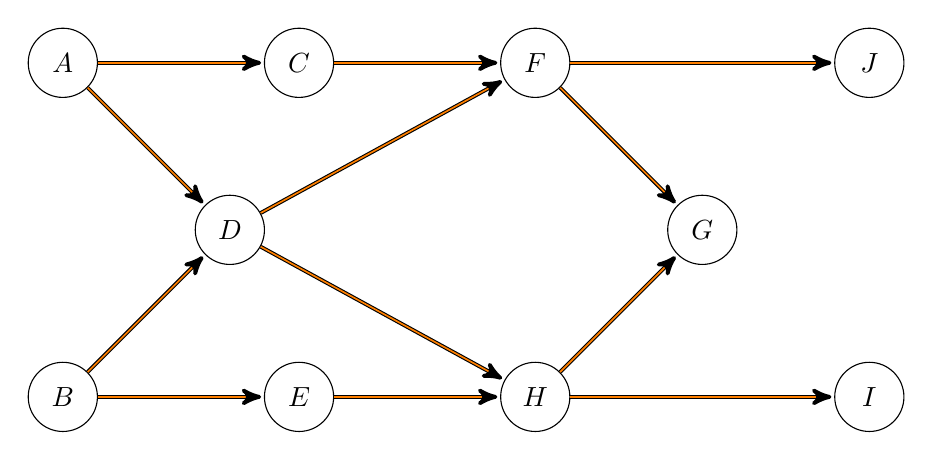
\begin{tikzpicture}[>=stealth',shorten >=1pt,node distance=3cm,on grid,initial/.style    ={}][!hb]
  \node[state]          (A)                        {$A$};
  \node[state]          (C) [right =of A]    {$C$};
  \node[state]          (D) [below right =of A]    {$D$};
  \node[state]          (B) [below left =of D]          {$B$};
  \node[state]          (E) [ right =of B]    {$E$};
  \node[state]          (F) [right =of C]    {$F$};
  \node[state]          (G) [below right =of F]    {$G$};
  \node[state]          (H) [right =of E]    {$H$};
  \node[state]          (I) [below right =of G]    {$I$};
  \node[state]          (J) [above right =of G]    {$J$};

\tikzset{mystyle/.style={->,double=orange}} 
\tikzset{every node/.style={fill=white}} 
\path (A)     edge [mystyle] (C)
      (A)     edge [mystyle] (D) 
      (B)     edge [mystyle] (E)
      (B)     edge [mystyle] (D)
      (C)     edge [mystyle] (F)
      (D)     edge [mystyle] (F)
      (D)     edge [mystyle] (H)
      (E)     edge [mystyle] (H)
      (H)     edge [mystyle] (G)
      (F)     edge [mystyle] (G)
      (F)     edge [mystyle] (J)
      (H)     edge [mystyle] (I); 
\end{tikzpicture}
\begin{enumerate}
    \item  What are the sources and sinks of the graph?
    \item  Give one linearization of this graph.
    \item  How many linearization does this graph have?
\end{enumerate}

% Manohar
\q{10}{} Consider the following directed graph.
\\\\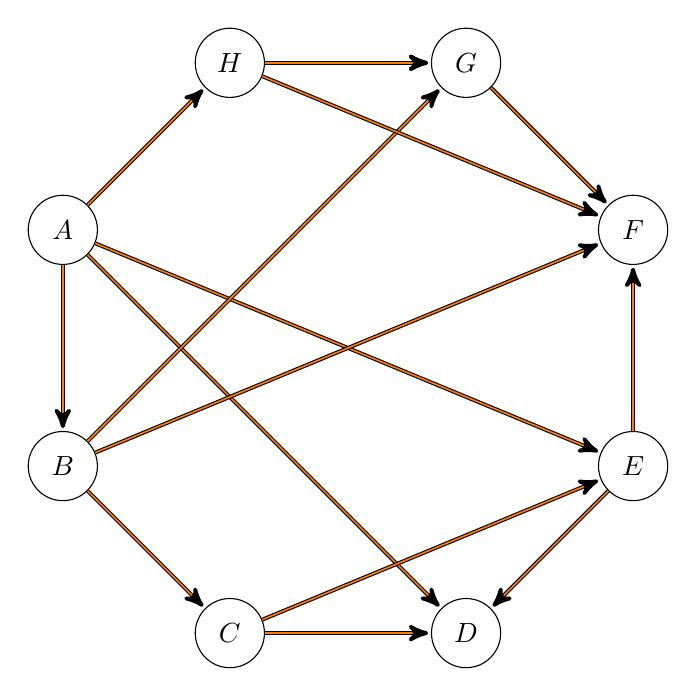
\begin{tikzpicture}[>=stealth',shorten >=1pt,node distance=3cm,on grid,initial/.style    ={}][!hb]
  \node[state]          (A)                        {$A$};
  \node[state]          (B) [below =of A]    {$B$};
  \node[state]          (C) [below right =of B]    {$C$};
  \node[state]          (D) [right =of C]          {$D$};
  \node[state]          (E) [above right =of D]    {$E$};
  \node[state]          (F) [above =of E]    {$F$};
  \node[state]          (G) [above left =of F]    {$G$};
  \node[state]          (H) [left =of G]    {$H$};

\tikzset{mystyle/.style={->,double=orange}} 
\tikzset{every node/.style={fill=white}} 
\path (A)     edge [mystyle] (B)
      (A)     edge [mystyle] (D) 
      (A)     edge [mystyle] (E)
      (B)     edge [mystyle] (C)
      (B)     edge [mystyle] (G)
      (B)     edge [mystyle] (F)
      (C)     edge [mystyle] (E)
      (C)     edge [mystyle] (D)
      (E)     edge [mystyle] (D)
      (E)     edge [mystyle] (F)
      (H)     edge [mystyle] (F)
      (H)     edge [mystyle] (G)
      (G)     edge [mystyle] (F)
      (H)     edge [mystyle] (G)
      (A)     edge [mystyle] (H); 
\end{tikzpicture}

\begin{enumerate}
    \item  Perform depth-first search with timing (DFS-with-timing) on the above graph; whenever there’s a choice of vertices, pick the one that is alphabetically first: give the pre and post number of each vertex.
    \item  Draw the meta-graph of this graph, and give the vertices in each connected component.
\end{enumerate}

% Manohar
\q{10}{}
You are in charge of the United States Mint. The money-printing machine has developed a strange bug: it will only print a bill if you give it one first. If you give it a d-dollar bill, it is only willing to print bills of
value $d^2 \mod 400$ and $d^2 +1 \mod 400$. For example, if you give it a \$6 bill, it is willing to print \$36 and
\$37 bills, and if you then give it a \$36-dollar bill, it is willing to print  \$96 and \$97. %(1296 (mod 400) = 96.)

You start out with only a \$1 bill to give the machine. Every time the machine prints a bill, you are allowed to give that bill back to the machine, and it will print new bills according to the rule described above. You
want to know if there is a sequence of actions that will allow you to print a \$20 bill, starting from your \$1 bill. Model this task as a graph problem: give a precise definition of the graph (what are the vertices and edges) involved and state the specific question about this graph that needs to be answered. Give an algorithm to solve the stated problem and give the running time of your algorithm.

\end{qunlist}
\end{document}